\chapter{Program Synthesis}\label{chap:program-synthesis}


Program synthesis is a very wide field of research. It has been studied by several different research communities and applied to diverse problems. As such, many approaches have been proposed to deal with the specific challenges introduced by each application, resulting in a great variety of focused algorithms that aim at finding a better program in less time. In this chapter, we take a more in-depth look into some of these techniques.

In \autoref{sec:rel-sketching} we introduce sketch-based enumeration: an enumeration method that deals with partial programs. In \autoref{sec:cegis}, we look at a method that steers the search in the right direction by using information about wrong answers to avoid future similar mistakes.
%
In Sections~\ref{sec:ogis} and~\ref{sec:rel-user-interaction}, we look at ways to deal with the ambiguity of the desired behaviour specification in inductive synthesis.
%
Finally, in \autoref{sec:rel-regex-synthesizers}, we take an in-depth look at two existing regular expression synthesizers: \AlphaRegex and~\Regel.

\section{Sketch-based Enumeration}\label{sec:rel-sketching}

\begin{figure}
    \centering
    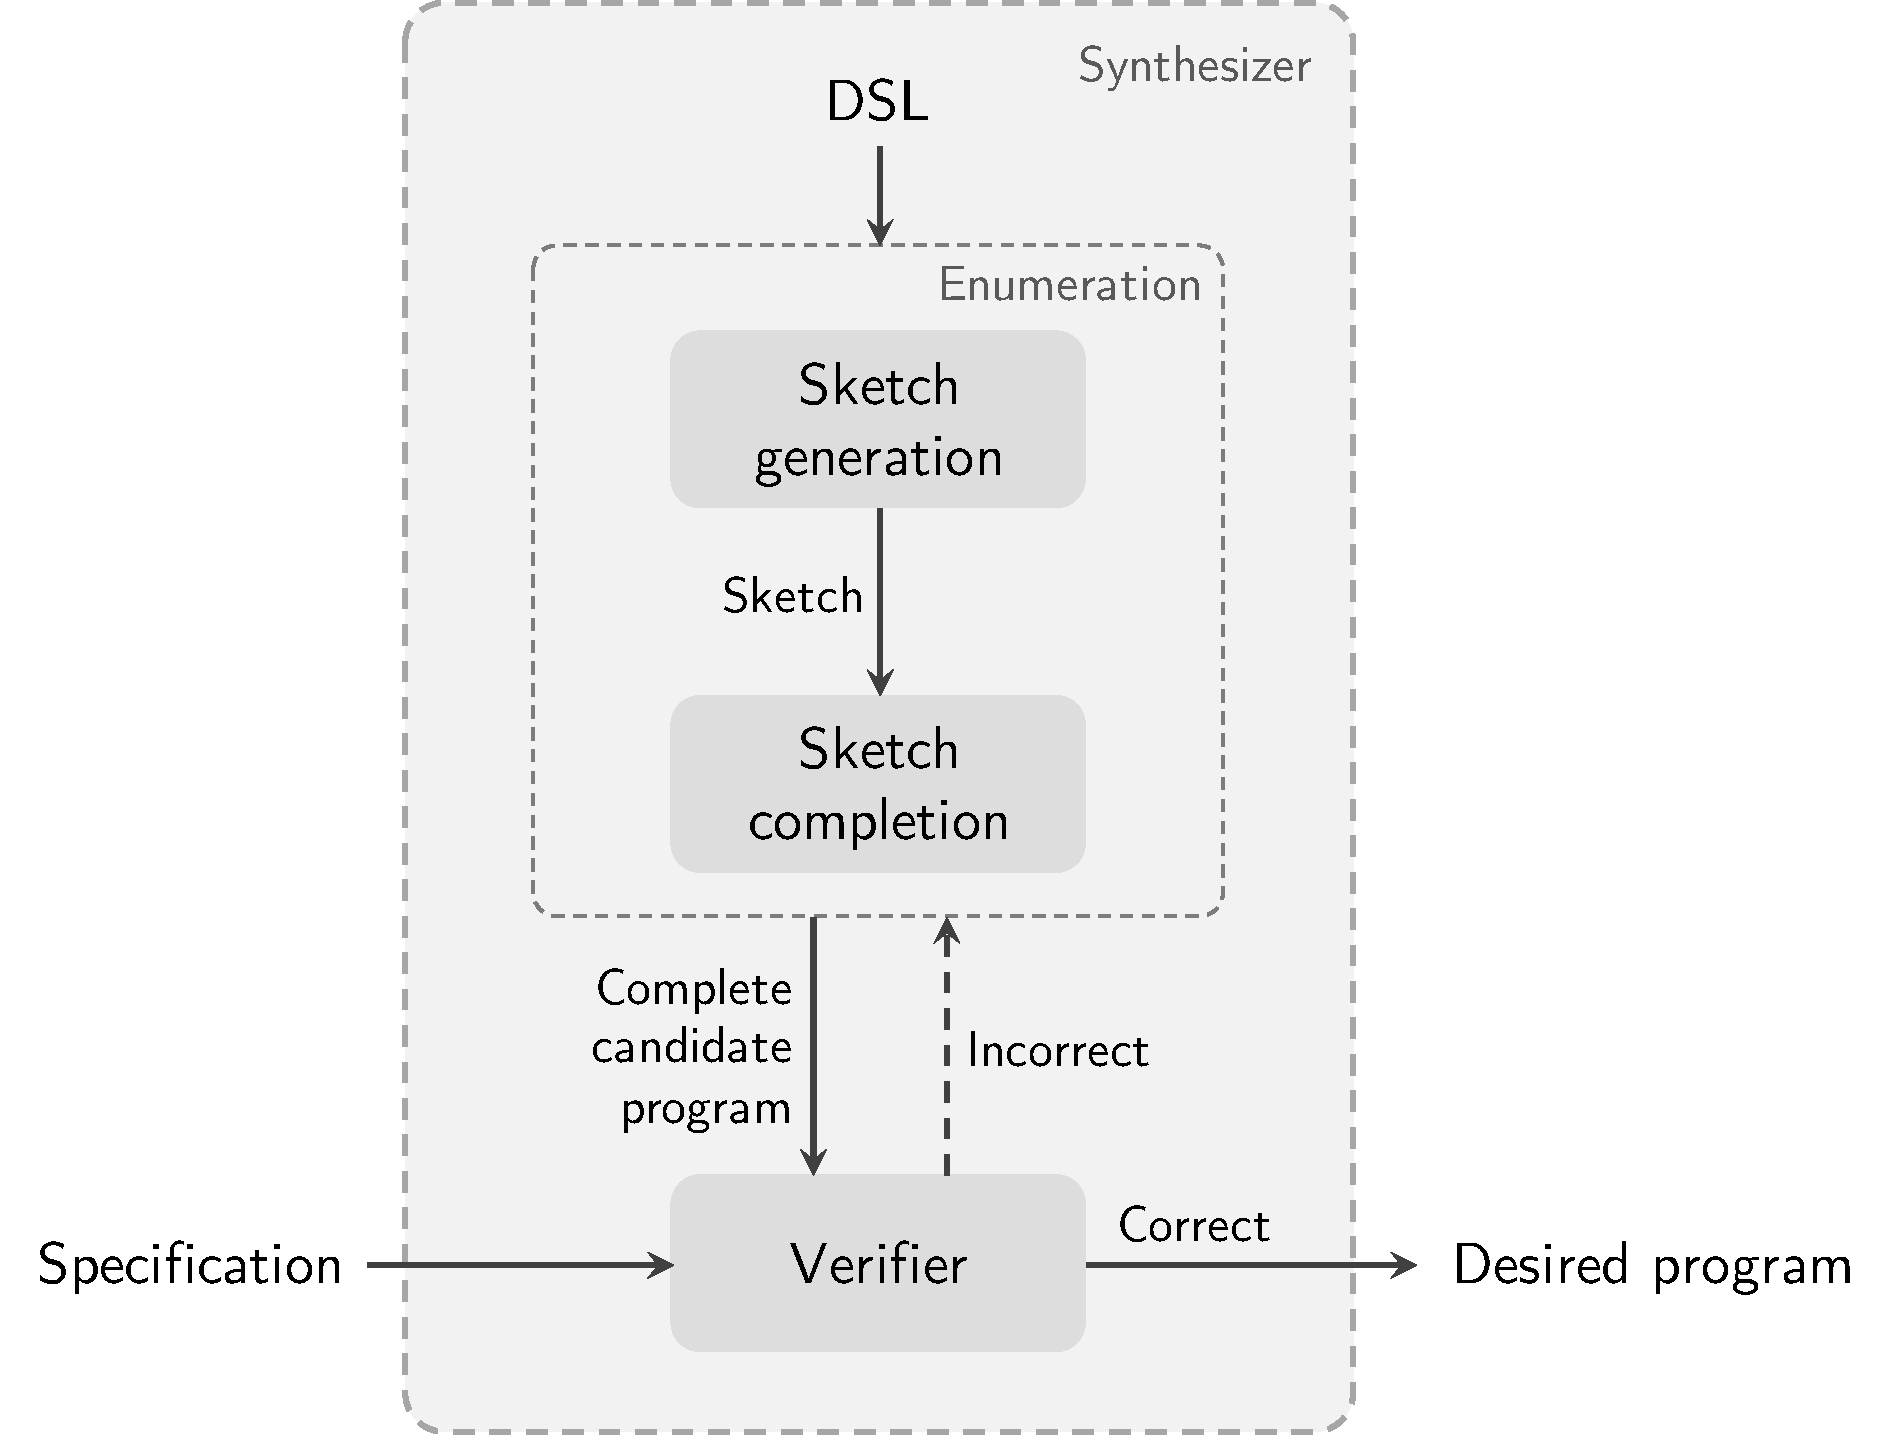
\includegraphics[scale=.35]{pictures/sketch.pdf}
    \caption{Sketch-based enumeration}
    \label{fig:sketch_enumeration}
\end{figure}

Some synthesizers perform enumerative search using partial programs \cite{Solar-LezamaPhDThesis,DBLP:conf/pldi/Solar-LezamaRBE05,DBLP:conf/asplos/Solar-LezamaTBSS06,DBLP:conf/pldi/WangCB17,DanielThesis,Regel20,DBLP:conf/pldi/FengMGDC17,DBLP:conf/popl/FengM0DR17,DBLP:journals/pacmpl/Yaghmazadeh0DD17,DBLP:journals/sttt/Solar-Lezama13}.
%Partial programs are a high-level representation of the intended program.
Instead of completely defining a program, partial (or incomplete) programs contain holes alongside the \ac{DSL} components. %, i.e., parts of the program that refer to lower-level implementation details.
For a partial program to become a syntactically correct complete program, all its holes must be filled with syntactically consistent expressions.
%
If we think in terms of the \ac{DSL}'s representation as a \ac{CFG}, a \textit{complete} program is a production of the grammar containing only terminal symbols, i.e, only operators and literal values in the \ac{DSL}. In contrast, a \textit{partial} program is a production of the grammar that may contain non-terminal symbols. Since each non-terminal symbol can correspond to many terminal symbols, a partial program can represent many complete programs.

Sketch-based enumeration deals with a particular type of partial programs: \textit{sketches}. A sketch is a partial program where the holes cannot be filled with operators: all missing constructs are literal values of the \ac{DSL}.
%
Instead of enumerating complete programs, a sketch-based synthesizer takes one of two approaches: Either
\begin{enumerate*}[label=(\roman*)]
    \item a sketch is provided by the user, who already possesses a high-level description of the desired program, in which case the synthesizer must complete it according to the specification, or
    \item the synthesizer is responsible for both producing a suitable sketch and completing it. The enumeration process is then split in two steps: sketch generation and sketch completion.
\end{enumerate*}
During sketch generation, the synthesizer enumerates incomplete programs in some order. During sketch completion, the synthesizer enumerates complete programs for each given sketch, by successively filling each hole with a syntactically correct expression. Sketch-based enumeration is outlined in \autoref{fig:sketch_enumeration}.

In many synthesizers, two-step enumeration outperforms normal enumeration because there is a very efficient way to fill the sketch holes, either because the few possible values exist for each hole, or because they can be directly deduced from the specification (instead of enumerated).



\section{\acl{CEGIS}}\label{sec:cegis}

Program synthesis is a search problem where the goal is to find a program \(P\) that satisfies a given specification \(\phi\).
\(\phi(\vec{x}, y)\) is \true{} if and only if \(y\) is the desired output value for input \(\vec{x}\).
We can define the program synthesis problem with the following logic formula:
%
\begin{equation}\label{eq:ps-2nd-order}
\exists P \; \forall \vec{x}, y : (P(\vec{x}) = y) \Rightarrow \phi(\vec{x}, y).
\end{equation}
%
\noindent
Due to the existential quantifier over function \(P\), \eqref{eq:ps-2nd-order} is a second-order formula and, as such, it is generally undecidable. 
To work around this problem, we may note that even though \textit{finding} a program that satisfies a specification may be infeasible, \textit{verifying} that a given program \(P\) satisfies a specification is a first-order problem:
%
\begin{equation}\label{eq:ps-1st-order}
\forall \vec{x}, y : (P(\vec{x}) = y) \Rightarrow \phi(\vec{x}, y).
\end{equation}
%
Formula \eqref{eq:ps-1st-order} is a first-order formula and can be solved using an off-the-shelf first-order solver. Any program \(P\) that satisfies~\eqref{eq:ps-1st-order} is a correct program, i.e., it complies with the specification \(\phi\).
Instead of proving \eqref{eq:ps-1st-order}, we can equivalently disprove its negation:
%
\begin{equation}\label{eq:counterexample}
\exists \vec{x}, y : (P(\vec{x}) = y) \wedge \neg \phi(\vec{x}, y).
\end{equation}
%
Formula \eqref{eq:counterexample} is also a first-order formula.
Formula~\eqref{eq:counterexample} is unsatisfiable if and only if \(P\) is a correct program.
Therefore, to find a correct program, we search the program space for a program \(P\) such that~\eqref{eq:counterexample} is unsatisfiable. Once found, \(P\) can be returned to the~user. %To achieve this, we can use enumerative search (previously explained in \autoref{sec:enum-search}), whose definition fits well into this way of verifying correctness of the program: the \textit{verifier} entity is then a solver that tries to satisfy formula~\eqref{eq:counterexample} (see Figures \ref{fig:enumerative-search} and~\ref{fig:CEGIS}).

\begin{figure}
    \centering
    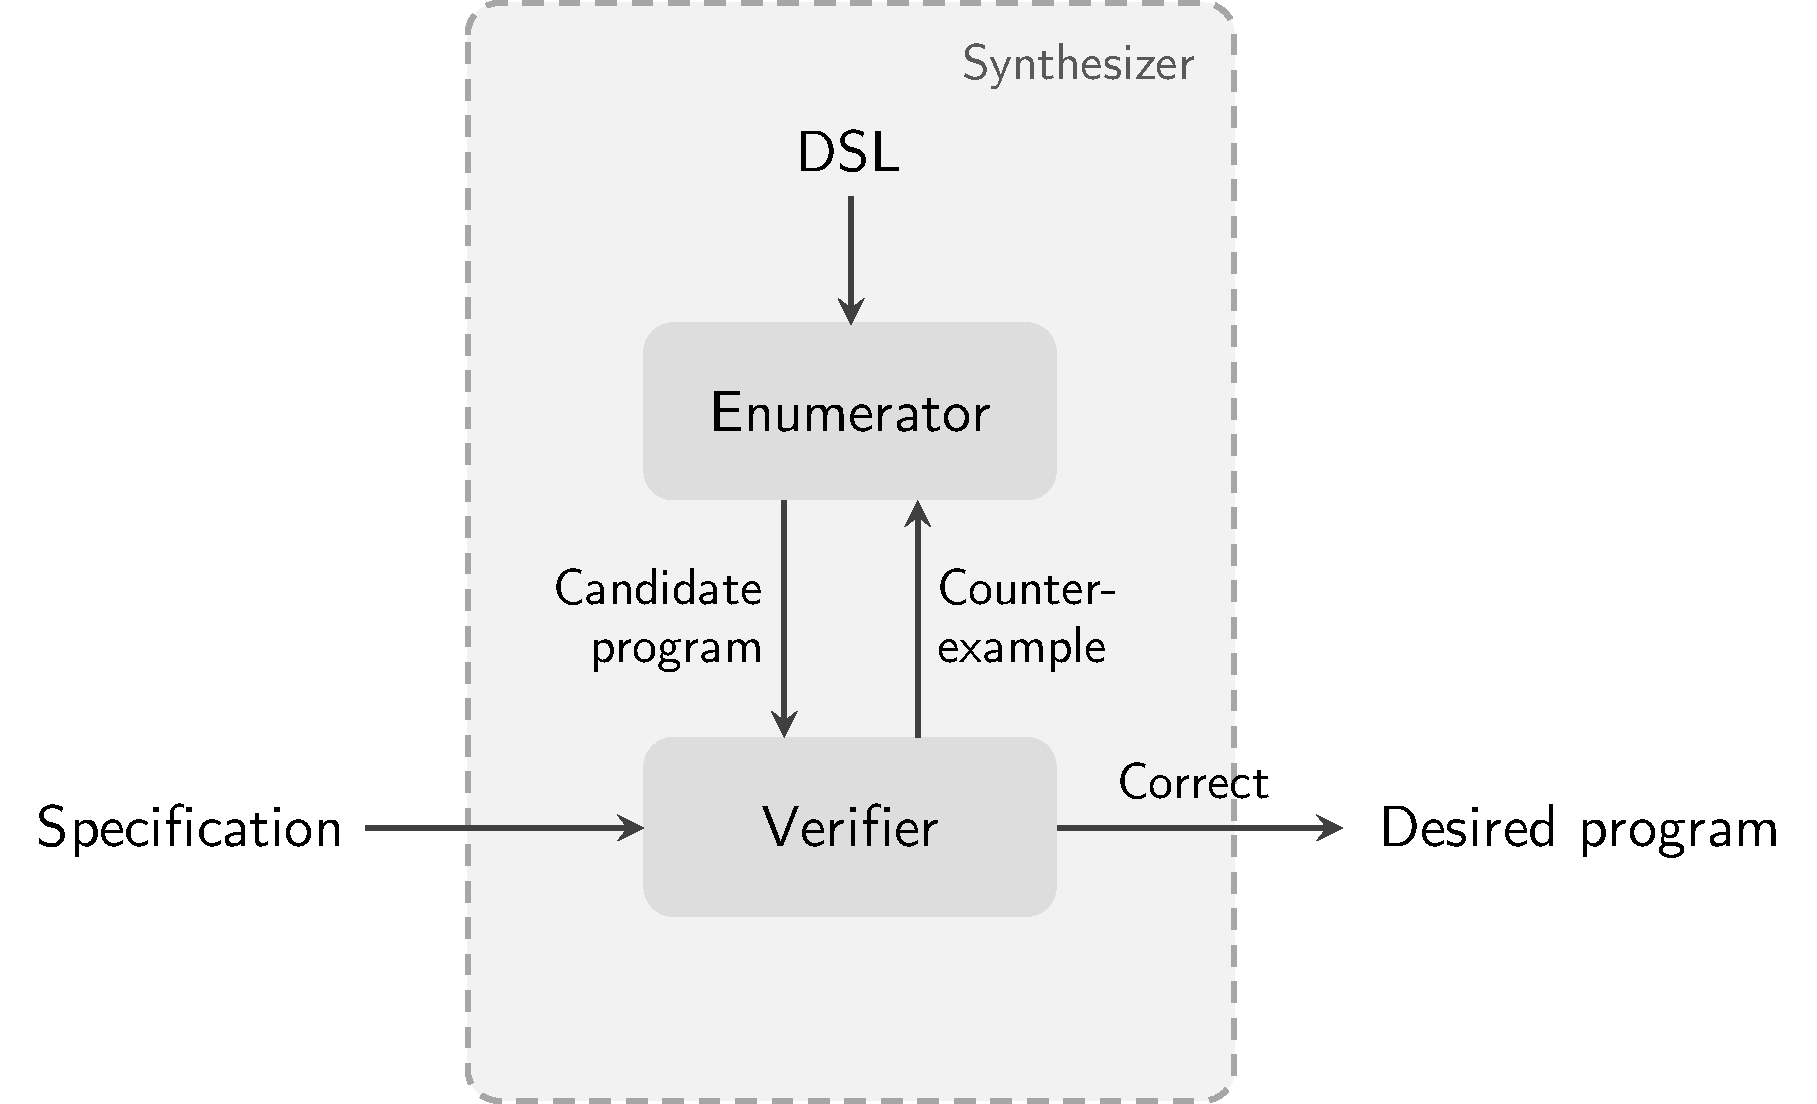
\includegraphics[scale=.35]{pictures/cegis.pdf}
    \caption{\ac{CEGIS}}
    \label{fig:cegis}
\end{figure}

Whenever we encounter a program \(P\) for which formula~\eqref{eq:counterexample} is satisfiable, the values of \(\vec{x}\) and \(y\) that satisfy the formula constitute a counterexample: an input \(\vec{x}\) for which \(P\) does not satisfy the specification \(\phi\); in other words, an input \(\vec{x}\) to which our program returns the wrong output.
If we take this counterexample \((\vec{x}, y)\) into account during our subsequent search, none of the new candidate programs returns \(y\) on the input \(\vec{x}\).
We have thus strengthened the specification, eliminating the previous incorrect candidate program.

\begin{definition}[Counterexample]
A counterexample \((\vec{x}, y)\) for an incorrect program \(P\) is an input-output pair such that \(P(x) = y\) and \(\neg \phi(\vec{x}, y)\), i.e., \(y\) is the output returned by \(P\) on input \(\vec{x}\) even though \((\vec{x}, y)\) is not consistent with the specification.
\end{definition}

This approach was proposed in \citeyear{Solar-LezamaPhDThesis} by \citeauthor{Solar-LezamaPhDThesis} in his PhD Thesis \cite{Solar-LezamaPhDThesis} and it is represented in \autoref{fig:cegis}. In this figure, the \textit{verifier} is a solver that tries to satisfy formula~(\ref{eq:counterexample}).

We can further improve this method by reformulating the verification formula in order to produce a constructive counterexample:
%
\begin{equation}\label{eq:constructive}
\exists \vec{x}, y : (P(\vec{x}) \neq y) \wedge \phi(\vec{x}, y).
\end{equation}
%
Like before, \eqref{eq:constructive} is a first-order formula and it is unsatisfiable if and only if \(P\) is a correct program.
When \eqref{eq:constructive} is satisfiable \(P\) is not a correct program and the values of \(\vec{x}\) and \(y\) that satisfy the formula are now a \textit{constructive} counterexample: \(y\) is the correct output for input \(\vec{x}\).
While a model \((\vec{x}, y)\) that satisfies \eqref{eq:counterexample} is an input-output pair that the program must \textit{not} satisfy, a model \((\vec{x}, y)\) that satisfies \eqref{eq:constructive} is a correct input-output pair that the program \textit{must} satisfy.
Adding the constructive counterexample to our previous specification results in a much stronger constraint and prunes the remaining search space even further. %However, this reformulation is only possible when there is only one output value that satisfies the specification for the input value~\(\vec{x}\).

\begin{definition}[Constructive counterexample]
A constructive counterexample \((\vec{x}, y)\) for an incorrect program \(P\) is an input-output pair such that {{\(P(x)~\neq~y\)}} and \(\phi(\vec{x}, y)\), i.e., \(y\) is not the output returned by \(P\) on input \(\vec{x}\) even though \((\vec{x}, y)\) is consistent with the specification.
\end{definition}

\section{\acl{OGIS}} \label{sec:ogis}
As discussed in \autoref{sec:desired-behaviour-spec}, \ac{PBE} comes with the drawback of incompleteness of the behaviour specification. Many programs are consistent with the provided specification, but not all these programs exhibit the user's intended behaviour.

In order to restore soundness of the solution, \citeauthor{DBLP:conf/icse/JhaGST10} proposed in \citeyear{DBLP:conf/icse/JhaGST10} a new approach which makes use of distinguishing inputs to disambiguate the input-output examples: \acf{OGIS}~\cite{DBLP:conf/icse/JhaGST10}.
An \textit{I/O~oracle} maps any given input to the desired output and it is used as an alternative to a complete specification. This means that whenever the \textit{I/O~oracle} is queried on any input vector \(\vec{x}\), it always returns the correct output \(y\).

We start with the same schema we had for \ac{CEGIS} (\autoref{fig:cegis}),  with a \textit{verifier} which, upon receiving a program \(P\), decides whether it is consistent with the behavioural constraints~\(\phi\). However, in \ac{OGIS} we no longer return to the user the first correct program we find.

When a correct program \(P_1\) is found, it is stored, and the search continues for another correct program. If no other correct program is found, then \(P_1\) is the unique correct program and it can be returned to the user. If another correct program \(P_2\) is found, then we have two programs consistent with the provided specification, i.e., \(P_1\) and \(P_2\) satisfy the following formulas:
%
\begin{subequations}
\begin{equation}
  \forall \vec{x}, y : (P_1(\vec{x}) = y) \Rightarrow \phi(\vec{x}, y),
\end{equation}
\begin{equation}
  \forall \vec{x}, y : (P_2(\vec{x}) = y) \Rightarrow \phi(\vec{x}, y).
\end{equation}
\end{subequations}

\noindent
Upon finding two correct programs, we want to find an input to which the two programs \(P_1\) and \(P_2\) return different outputs: a \textit{distinguishing input}. To produce a distinguishing input, we can try to solve:
%
\begin{equation}\label{eq:distinguishing}
  \exists \vec{x}: P_1(\vec{x}) \ne P_2(\vec{x}).
\end{equation}
%
If formula~(\ref{eq:distinguishing}) is unsatisfiable then \(P_1\) and \(P_2\) are equivalent programs.
In this case, either there are more correct programs that can be taken into consideration, or \(P_1 = P_2\) is the unique program that satisfies all input-output examples and it is returned to the user.
If~(\ref{eq:distinguishing}) is satisfiable, the distinguishing input \(\vec{x}\) can be extracted from the model \((\vec{x}, y_1, y_2)\) that satisfies it.
Once found, we can query the \textit{I/O oracle} on the distinguishing input, who yields the correct output for it.
The distinguishing input along with its correct output forms a new correct input-output pair \((\vec{x}, y)\) which can then be added to the specification~\(\phi\), further constraining the search space.

In the end of this cycle, we have a set of input-output pairs that completely specify the generated program, thus eliminating all ambiguity.

\begin{figure}
    \centering
    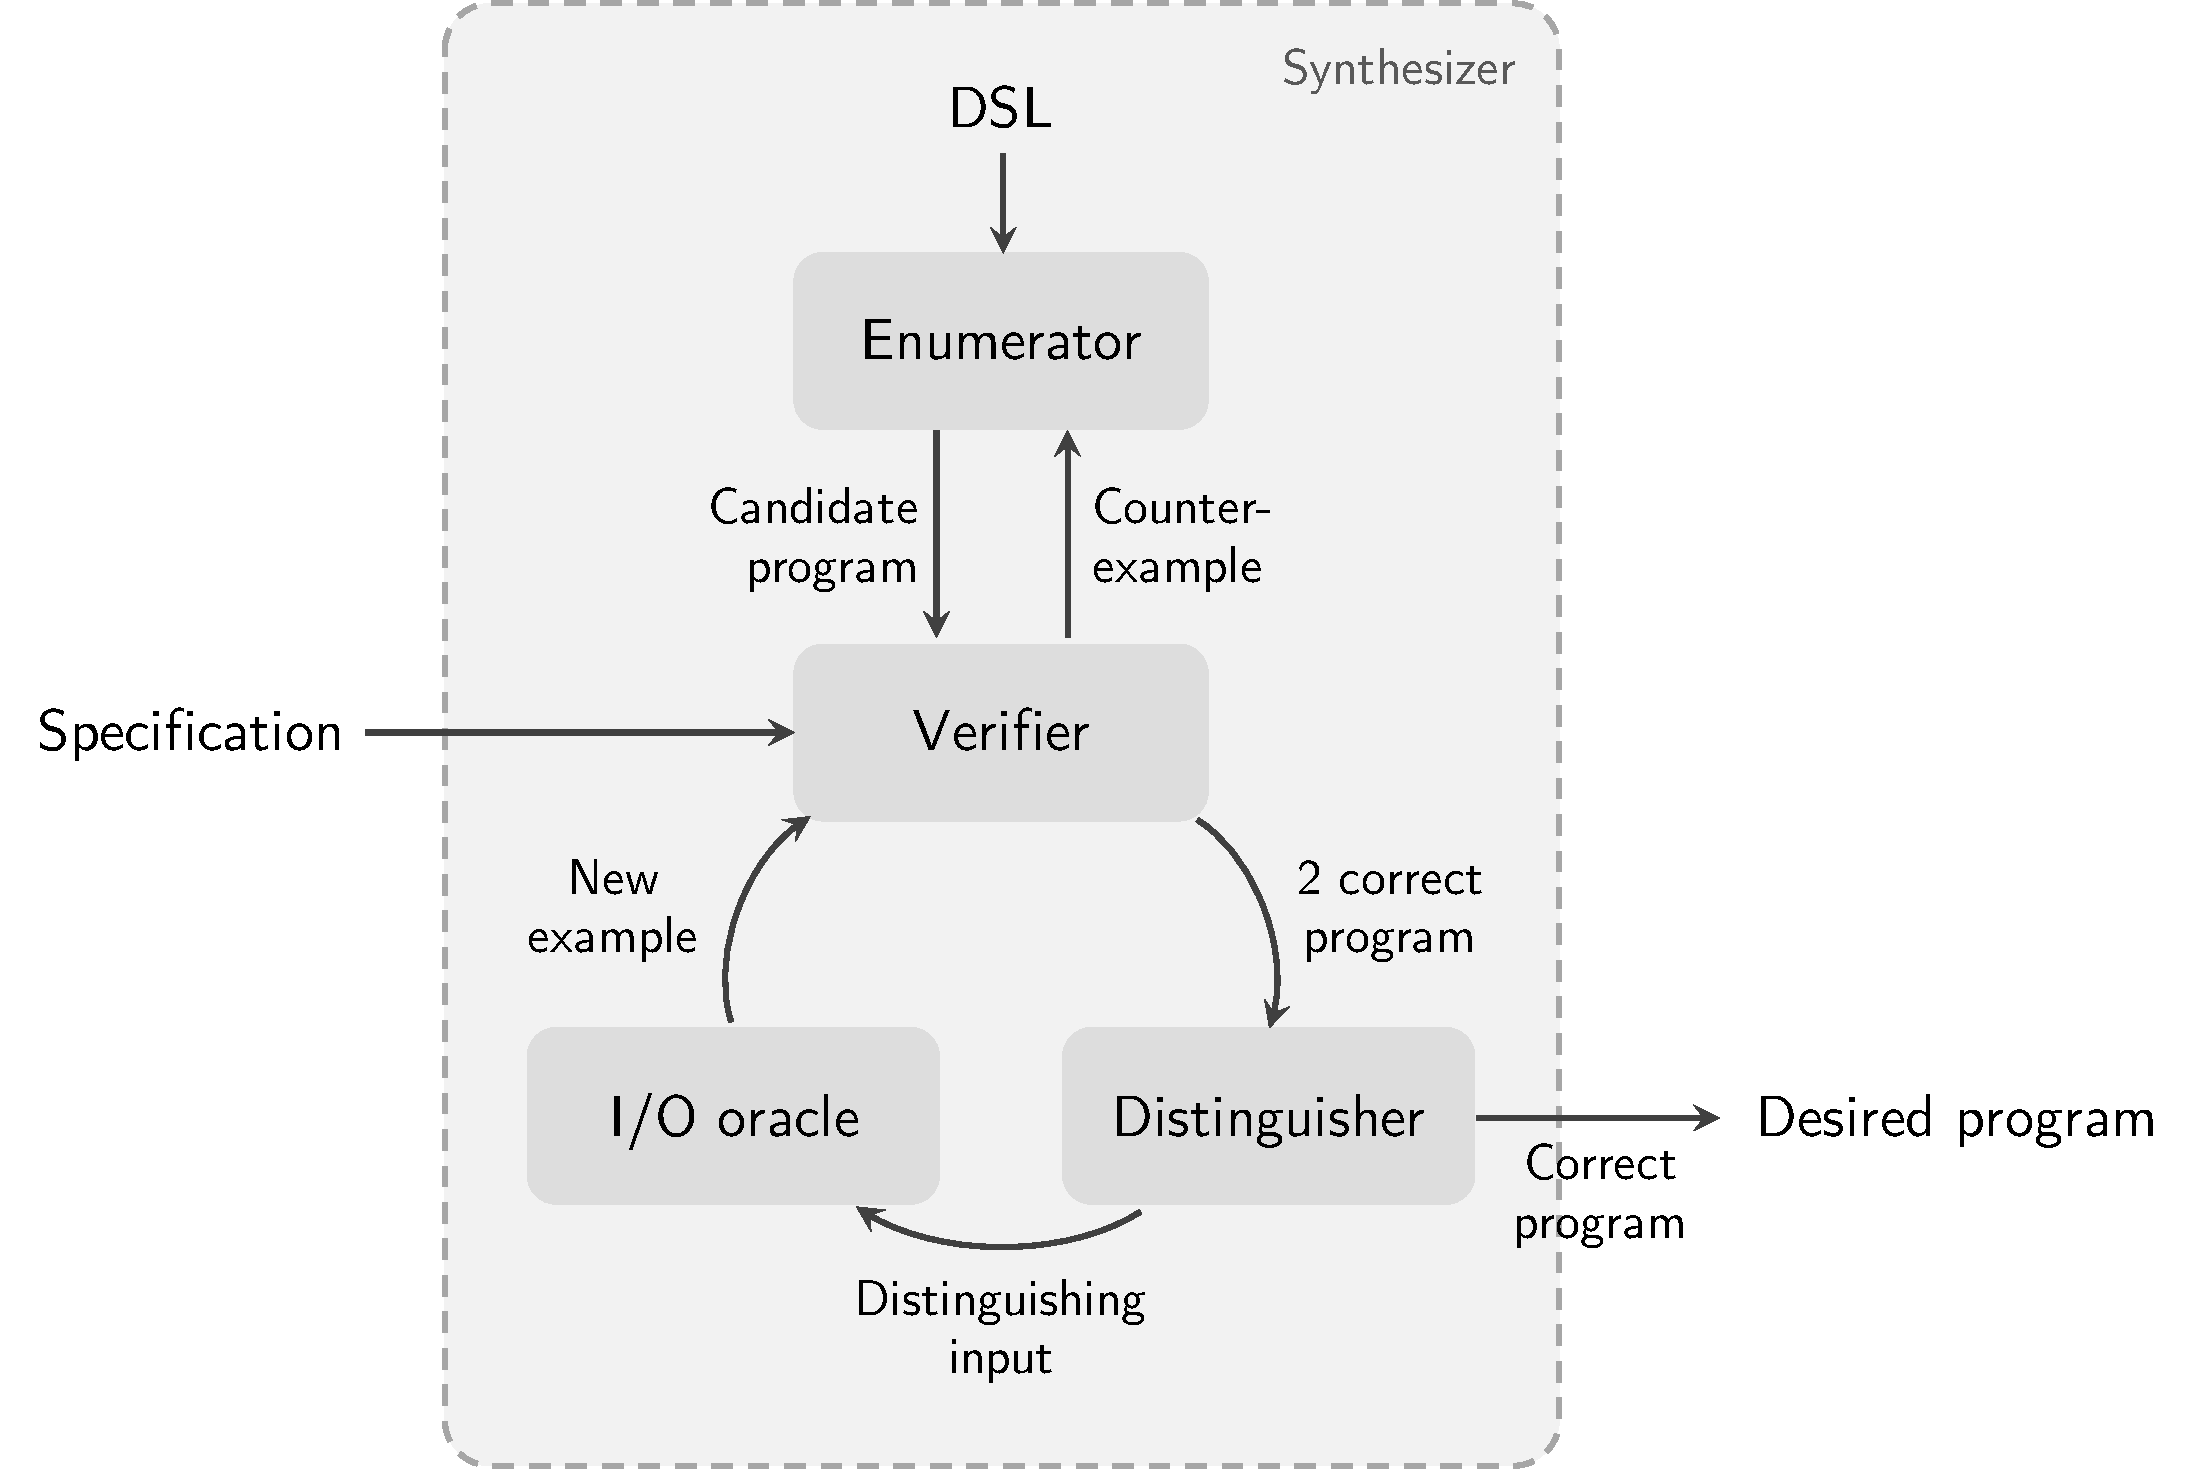
\includegraphics[scale=.35]{pictures/ogis.pdf}
    \caption{\ac{OGIS}}
    \label{fig:ogis}
\end{figure}

This method is illustrated in \autoref{fig:ogis}. In this figure, the \textit{enumerator} and \textit{verifier} are identical to those in \ac{CEGIS} (\autoref{fig:cegis}). The \textit{distinguisher} is a new entity, which can be a solver that tries to satisfy formula~(\ref{eq:distinguishing}).


\section{User Interaction} \label{sec:rel-user-interaction}

As mentioned before, \ac{PBE} uses input-output examples as the desired behaviour specification, which can be very ambiguous. When the synthesizer simply picks a correct program to return to the user, it may not satisfy the desired behaviour in corner cases not covered by the examples provided.
In order to increase confidence in the synthesizer's solution, a good way to disambiguate the specification is by explicitly interacting with the user so he or she can provide further information about the intended~program.
In this section we look at a few different user interaction models that allow the synthesizer to gather more information about the intended program, thus resolving the ambiguity in the initially provided examples.

\subsection{Conversational Clarification Model}\label{sec:rel-conv-clarification}
\begin{figure}
    \centering
    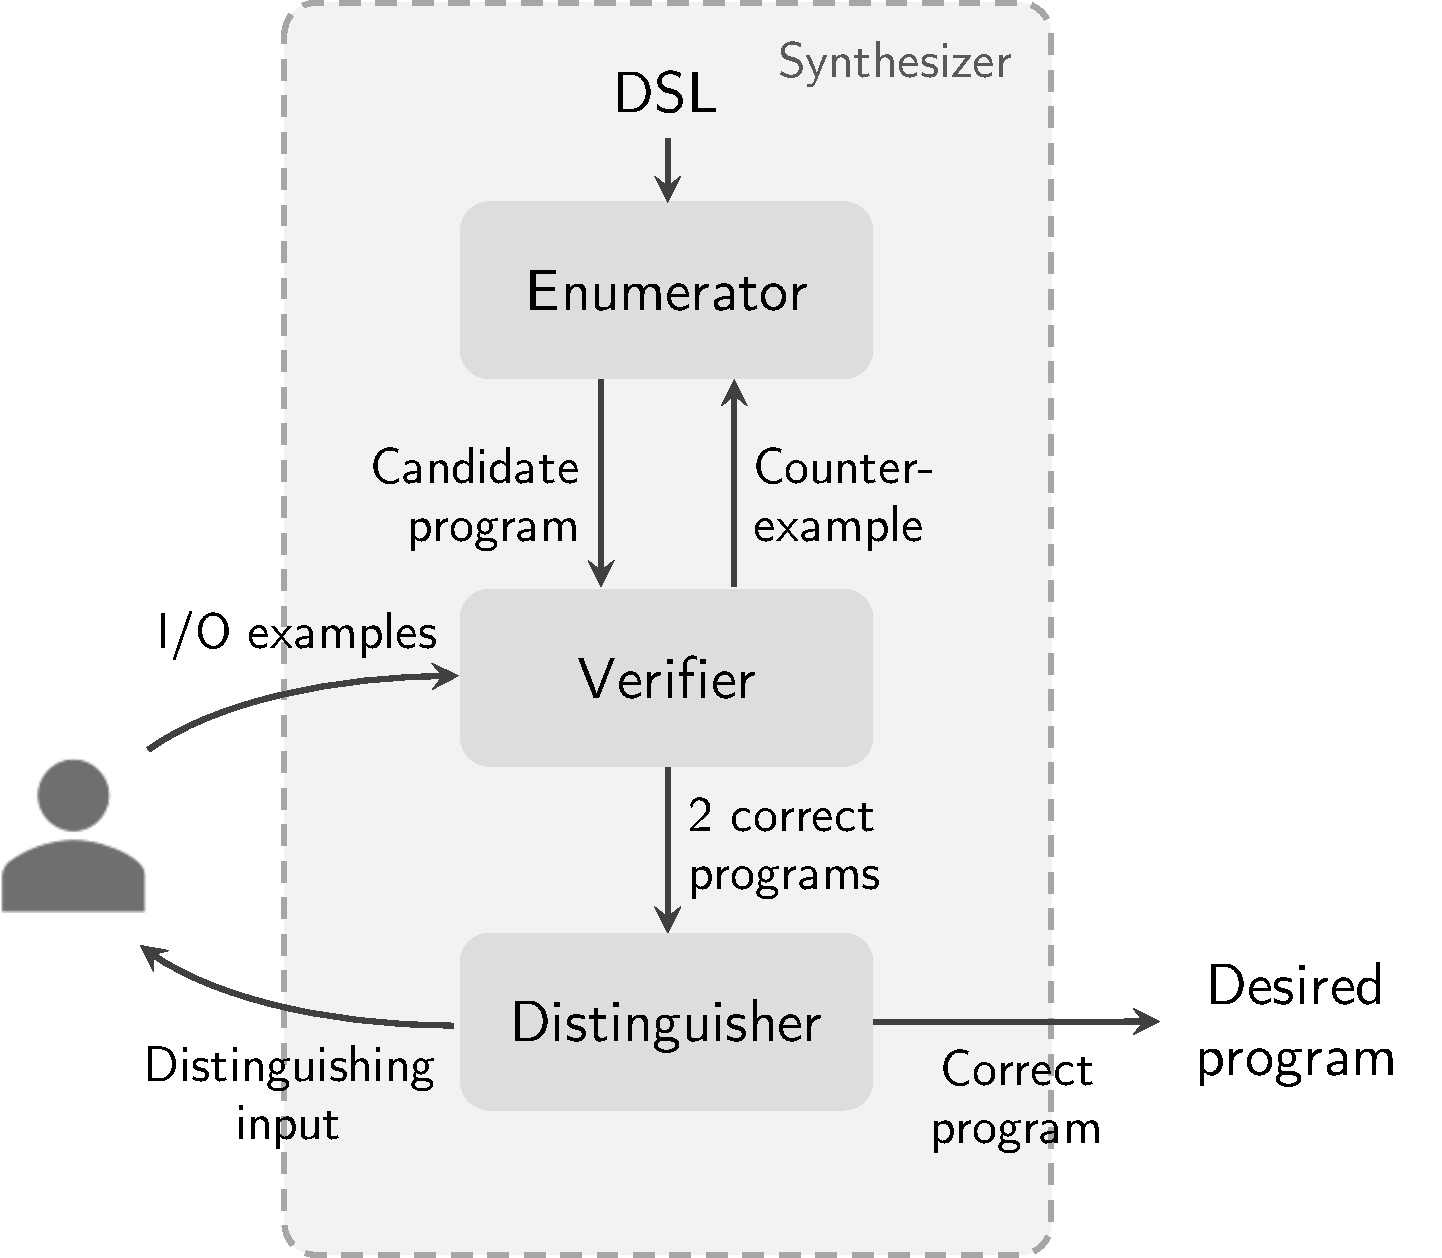
\includegraphics[scale=.35]{pictures/conversational_clarification.pdf}
    \caption{Conversational clarification}
    \label{fig:conversational_clarification}
\end{figure}

Conversational clarification is an interaction method first described in \citeyear{DBLP:conf/uist/MayerSGLMPSZG15} by \citet{DBLP:conf/uist/MayerSGLMPSZG15} that has since been successfully integrated in many synthesizers  \cite{DBLP:journals/pvldb/LiCM15,DBLP:journals/corr/abs-1909-11206,DBLP:conf/sigmod/WangCB17,DBLP:conf/pldi/WangCB17}.
During the synthesis procedure, the synthesiser asks the user questions about certain inputs, and uses the answers to resolve ambiguities in the desired behaviour specification. 

After the synthesizer has generated several programs that are consistent with the user-provided examples, it uses the \textit{distinguisher} described in \autoref{sec:ogis} to produce a distinguishing input:
an input for which two correct programs yield two different outputs.
The synthesizer then queries the user on what is the desired output for that specific input (it may be the output returned by one of the synthesised programs, or a different one altogether).
The distinguishing input along with the desired output form a new input-output example, which is added to the specification, making it stronger.
Each distinguishing input splits the search space in a different way, so the number of necessary user interactions depends on the chosen distinguishing input in each iteration.
In the end, only one program remains. Since all ambiguity in the original specification has been resolved, the remaining program is the desired program and it can be returned to the user.

Conversational clarification is represented in \autoref{fig:conversational_clarification}. It is no more than a variation of the \ac{OGIS} method, described in \autoref{sec:ogis}, where the user plays the part of the \textit{I/O oracle}.


\subsection{\optmodel Model}\label{sec:rel-ramos-interaction}

\citeauthor{UnchartIt20}~\cite{UnchartIt20,unchartit-webpage} propose two interaction models: \optmodel and \ynmodel.
Both models have in common with conversational clarification the fact that they interact with the user using distinguishing inputs, i.e., new inputs generated by the synthesizer whose output differs for different candidate programs. 
The main difference is that, while conversational clarification distinguishes only between two programs, \optmodel and \ynmodel distinguish \textit{optimally} between \(n > 2\) candidate programs, \(P_1, ..., P_n\).
In each interaction they maximise the number of programs that are eliminated from the search space. Besides, unlike conversational clarification, with \optmodel and \ynmodel, the program's output is always shown to the user beforehand.
The user just has to select one among several or classify it as correct or incorrect.
In sum, not only are \optmodel and \ynmodel's interactions fewer, they are also easier for the user to answer.\footnote{\UnchartIt's interaction models can be tried out at \url{http://sat.inesc-id.pt/unchartit/dist/}}

The \optmodel model shows the user a distinguishing input, as well as several options that correspond to the outputs of candidate programs for that input. Then, the user selects the correct output among the provided options.
%If the selected output still corresponds to the output of several candidate programs, additional rounds of questions are performed to disambiguate solely among those programs.
Ideally, there is a single input example that produces a different output for each candidate program.
In this best-case scenario, a single interaction is sufficient to disambiguate all candidate programs with the \optmodel model: only one is consistent with the user's selection.

To produce the distinguishing input, \(\vec{x}\), we start by defining a Boolean variable \(b_{ij}\) for each pair \(i,j\in\{1, ..., n\},i<j\). \(b_{ij}\) is \true if and only if \(P_i\) and \(P_j\) have the same output for \(\vec{x}\):
%
\begin{equation}
    \bigwedge_{i,j \in \{1, ..., n\}, i < j} (P_i(\vec{x}) = P_j(\vec{x})) \leftrightarrow b_{ij}.
\end{equation}
%
To ensure that at least two of the candidate programs produce a different output for the distinguishing input \(\vec{x}\), we include the constraint:
%
\begin{equation}
    \bigvee_{i,j \in \{1, ..., n\}, i < j} \neg b_{ij}.
\end{equation}
%
Finally, since it is our goal to find an input such that all programs have different outputs, we want as few \(b_{ij}\) set to \true as possible.
Thus, we add the following soft constraints:
%
\begin{equation}
    \bigwedge_{i,j \in \{1, ..., n\}, i < j} \neg b_{ij}.
\end{equation}

We use a \ac{MaxSMT} solver to try and find a model that satisfies the formula. If it is unsatisfiable, then there is no input \(\vec{x}\) to which any of the programs have a different output, i.e., \(P_1, ..., P_n\) are all equivalent. If it is satisfiable, then we show \(\vec{x}\) to the user along with all possible outputs \(P_i(\vec{x})\). The user selects the correct output, and the synthesizer discards all programs whose output for \(\vec{x}\) differs.

\subsection{\ynmodel Model}

On the \ynmodel interaction model, the goal is to identify a distinguishing input \(\vec{x}\) that splits the set of programs into two sets \set{A} and \set{B}, such that all programs in \set{A} produce the same output \(o\)  given input \(\vec{x}\), and all programs in \set{B} produce outputs different than \(o\) given input \(\vec{x}\).
%
The goal is then to find \(\vec{x}\) such that half the programs are placed in each set.

To encode this problem into \ac{MaxSMT}, we have the same Boolean variables \(b_{ij}\) for all pairs \(i,j \in \{1, ..., n\}, i < j\), which are \true if and only if \(P_i\) and \(P_j\) have the same output for input \(\vec{x}\):
\begin{equation}
    \bigwedge_{i,j \in \{1, ..., n\}, i < j} (P_i(\vec{x}) = P_j(\vec{x})) \leftrightarrow b_{ij}.
\end{equation}
%
Then, we define a set of Boolean variables \(p_i^\set{A}\) (resp. \(p_i^\set{B}\)) for all \(i\in \{1, ..., n\}\) which are assigned \true if and only if program \(P_i\) is placed in set \set{A} (resp. \set{B}).
%
If two candidate programs \(P_i\) and \(P_j\) produce the same output for \(\vec{x}\) (i.e. \(b_{ij}\) is \true), then \(P_i\) and \(P_j\) must be placed in the same set. On the other hand, if two programs produce different outputs (i.e. \(b_{ij}\) is \false), then only one of them can be placed in set \set{A}. Finally, each program must be placed in one and only one set. To enforce this, we add the constraints:
\begin{equation}
    \bigwedge_{i,j \in \{1, ..., n\}, i < j} b_{ij} \rightarrow \left( (p_i^\set{A} \wedge p_j^\set{A}) \vee (p_i^\set{B} \wedge p_j^\set{B}) \right),
\end{equation}
%
\begin{equation}
    \bigwedge_{i,j \in \{1, ..., n\}, i < j} \neg b_{ij} \rightarrow (\neg p_i^\set{A} \vee \neg p_j^\set{A}), \; \textrm{and}
\end{equation}
%
\begin{equation}
    \bigwedge_{i \in \{1, ..., n\}} p_i^\set{A} \ne p_i^\set{B}.
\end{equation}
%
To ensure we have at least one program in set \set{A}, we add the constraint:
\begin{equation}
    %\sum_{i=1}^n p_i^B  \le n-1.
    \bigvee_{i \in \{1, ..., n\}} p_i^\set{A}.
\end{equation}

\noindent
Ideally, we would like \set{A} and \set{B} to have the same number of elements, so that when the user classifies \(\vec{x}\) as either correct or incorrect we can eliminate half the programs from the search space. To achieve this, we add the optimisation objective:
\begin{equation}
    \textrm{min.} \left|\sum_{i=1}^n p_i^A - \sum_{i=1}^n p_i^B \right|.
\end{equation}

As before, we use a \ac{MaxSMT} solver to solve the formula.
If the formula is unsatisfiable, then all programs are equivalent and there is no distinguishing input. In this case we can keep only one program and discard the rest.
If the formula is satisfiable, then the model assignment for \(\vec{x}\) is the distinguishing input. In this situation, the synthesizer shows \(\vec{x}\) to the user, along with the output of any program in \set{A} run with input \(\vec{x}\) (they all have the same output).
Finally, we ask the user if this is the desired output for input \(\vec{x}\). If the output is correct, we can eliminate from the search space all programs in \set{B}. Otherwise, we remove all programs in \set{A}.

\section{Regex Synthesizers}\label{sec:rel-regex-synthesizers}

In this section, we discuss prior work on the synthesis of regular expressions that is most closely related to our approach.
%
Previous approaches that perform general string processing~\cite{DBLP:conf/popl/Gulwani11,Fidex16} restrict the form of the regular expressions that can be synthesised. In contrast, we support a wide range of regular expressions operators, including the Kleene closure, positive closure, option, and range. 
%
More recent work that targets the synthesis of regexes is done by \AlphaRegex~\cite{AlphaRegex16} and \Regel~\cite{Regel20}.

\AlphaRegex performs an enumerative search and uses under- and over-approximations of regexes to prune the search space. However, \AlphaRegex is limited to the binary alphabet and does not support the kind of regexes that we need to synthesise for form validations. \AlphaRegex is analysed in depth in \autoref{sec:alpharegex}.


\Regel is a state-of-the-art synthesizer of regular expressions based on a multi-modal approach that combines input-output examples with a natural language description of user intent. They use natural language to build sketches that capture the high-level structure of the regex to be synthesised and subsequently use the input-output examples to fill those sketches. 
\Regel prunes the search space by using \AlphaRegex-like under- and over-approximations and symbolic regexes combined with SMT-based reasoning.

There are other approaches that synthesise regexes solely from natural language~\cite{DBLP:conf/naacl/KushmanB13,DBLP:conf/emnlp/LocascioNDKB16,DBLP:conf/emnlp/ZhongGYPXLLZ18}. We see these approaches as orthogonal to ours and expect that \Forest can be improved by hints provided by a natural language component such as was done in \Regel.
%
To the best of our knowledge, no previous work focused on the synthesis of conditions over capturing groups.


\subsection{\AlphaRegex}
\label{sec:alpharegex}
In \citeyear{AlphaRegex16}, \citet{AlphaRegex16} presented \AlphaRegex, a \ac{PBE} synthesizer of regular expressions in the binary alphabet, \(\Sigma = \{0, 1\}\).
%
Like with \Forest, with \AlphaRegex the user describes the desired accepted language by providing a set of positive and negative examples. The synthesised regular expression must define a language that includes all the positive examples and none of the negative ones.
\AlphaRegex uses an enumerative search technique, with a ranking method that prioritises simpler expressions.

The algorithm starts by examining the simplest regular expressions, \regex{0} and \regex{1}.
If these are not consistent with the examples, it checks more complex productions such as \regex{0|0}, \regex{0|1}, \regex{1|0}, \regex{1|1} (i.e. expressions in the form of \regex{\Box|\Box}), \regex{00}, \regex{01}, \regex{10}, \regex{11} (i.e. expressions in the form of \(\tt\Box\Box\)), and \regex{0*}, \regex{1*}, (i.e. expressions in the form of \(\tt\Box*\)).

Here, we introduce the hole (\(\Box\)), a placeholder for any regular expression. Regular expressions with or without holes are the states of the search.
The algorithm generates regular expressions by iteratively replacing holes with other states and checking if the resulting regular expressions are correct.

To speed up the search, \AlphaRegex makes use of three different kinds of search space pruning techniques: over-approximation, under-approximation and elimination of redundant states.

\paragraph{Over-approximation} is achieved by replacing holes in the current state with \regex{(0|1)*}.
This regular expression describes the language that accepts all the strings that can be written using the binary alphabet.
%The union of any  regular expression \(r\) with \regex{(0|1)*}, \(r|\tt(0|1)*\), is again \regex{(0|1)*}.
%The concatenation of any regular expression \(r\) with \regex{(0|1)*}, \(r\tt(0|1)*\), results in the original regular expression \(r\).
Therefore, over-approximation makes the state as general as it can be.
If the over-approximation rejects at least one of the positive examples we conclude that this state can never be used to build a solution.

\begin{example}
Consider the state \(\tt1\Box\), i.e., the concatenation of \regex{1} with a hole, which can be filled with any regular expression. The over-approximation of this state, \regex{1(0|1)*}, accepts all strings that a regular expression of the form \(\tt1\Box\) could possibly accept. Thus, if \regex{1(0|1)*} does not accept all the positive examples, this state is not worth considering, and can be pruned.
\end{example}

\paragraph{Under-approximation} consists in replacing holes in the current state with \regex{\emptyset}, the regular expression that corresponds to the empty language. The concatenation of any regular expression \(r\) with \(\tt\emptyset\), \(r\tt\emptyset\), results in \(\tt\emptyset\). The union of any  regular expression \(r\) with \(\tt\emptyset\), \(r|\tt\emptyset\), is the regular expression \(r\) itself.
If the under-approximation does not reject any of the negative examples,  we conclude that this state can never be used to build a correct solution.

\begin{example}
Consider now the state \(\tt1|\Box\), i.e., the union of \regex{1} with a hole. The under-approximation of this state, \(\tt1|\emptyset = 1\), restricts \regex{1|\Box} to the language that accepts as few strings as possible, in this case, the one containing only the string with a single `1'. If \regex{1} does not reject any of the negative examples, then this state can be pruned.
\end{example}

\paragraph{Elimination of redundant states} is done using the equivalences of regular expressions resulting from the algebraic rules of regular expressions.
%  described in \autoref{tab:regex-laws} in \autoref{sec:regex}
For example, the algorithm needs not evaluate the expression \(s\texttt{|}r\) if it has already considered \(r\texttt{|}s\), where \(r\) and \(s\) are regular expressions, as these expressions are equivalent.

\medskip

\noindent
The authors tested \AlphaRegex in 25 benchmark problems collected from textbooks on automata theory which are provided along with the code for their tool.
\AlphaRegex proved capable of synthesising relatively complex expressions, with more than a dozen operations, in under one minute.


\subsection{\Regel}

\begin{figure}
    \centering
    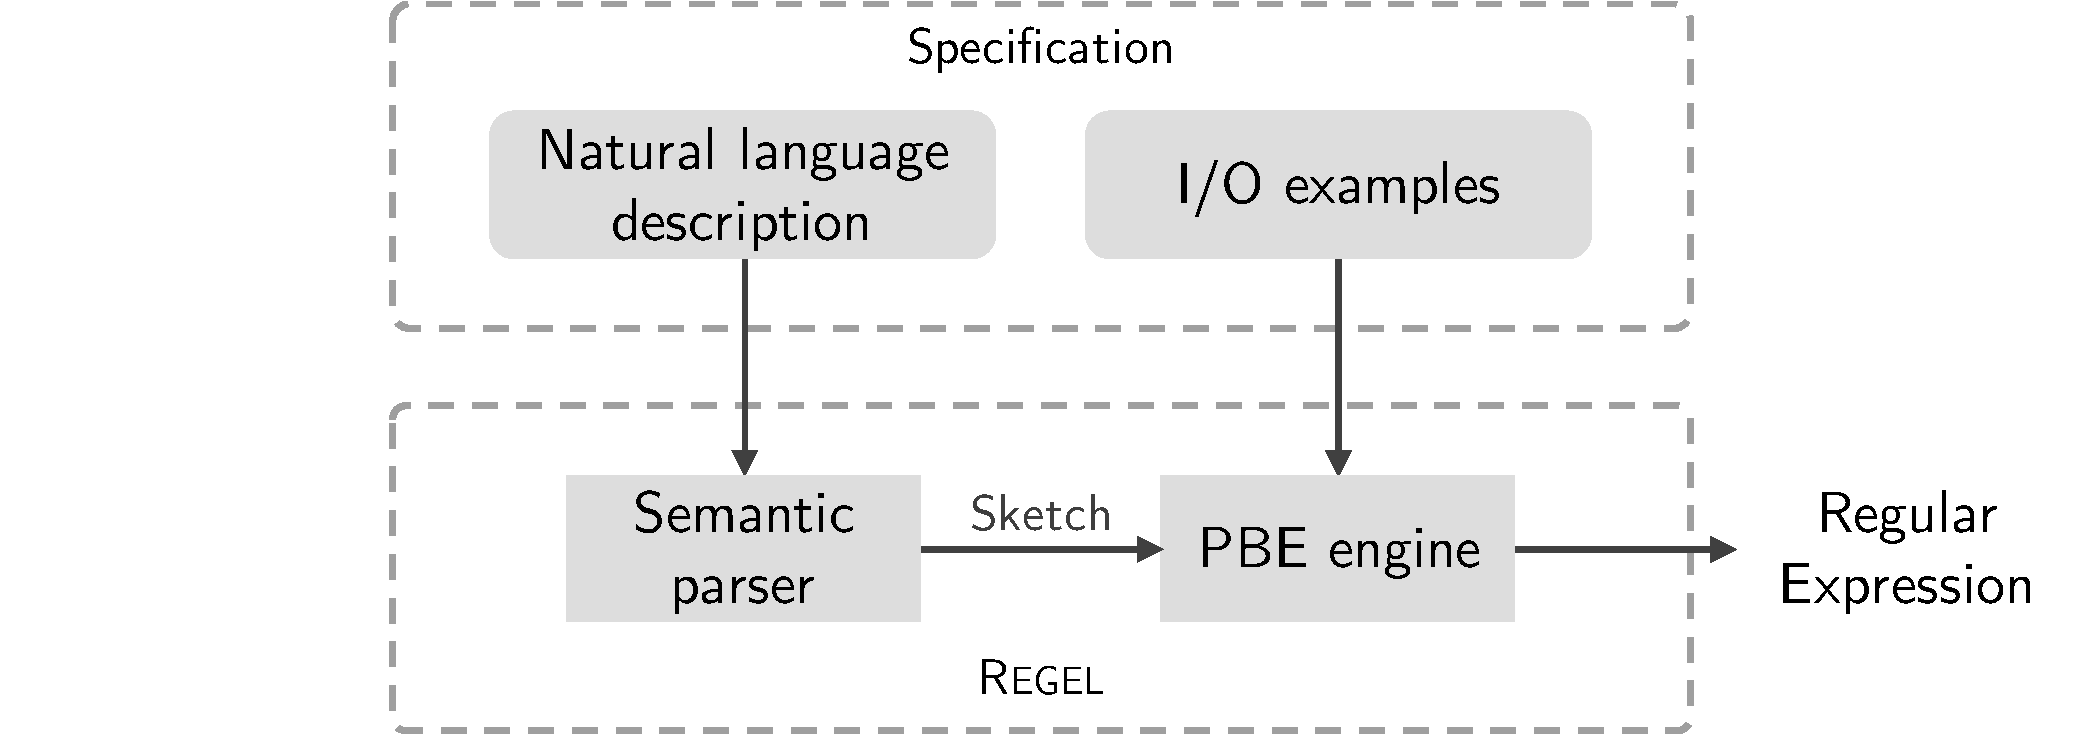
\includegraphics[scale=.35]{figures/regel.pdf}
    \caption{\Regel's synthesis pipeline}
    \label{fig:regel-synthesis}
\end{figure}

In \citeyear{Regel20}, \citet{Regel20} proposed \Regel, a multi-modal sketch-based regex synthesizer. \Regel accepts two different kinds of description of desired behaviour: 
\begin{enumerate*}[label=(\roman*)]
    \item a natural language description of the desired pattern (which is used to generate a sketch), and
    \item a set of positive and negative examples (which is used to complete the sketch).
\end{enumerate*}
\Regel's synthesis pipeline is shown in \autoref{fig:regel-synthesis}

\Regel's \ac{DSL} is a lot more expressive than that of \AlphaRegex. They synthesise common regex operators: concatenation, union, Kleene closure, positive closure, option and range. Besides the standard regex operators, they accept operations and (intersect) and not (complement), which are implemented at the automaton level.

\paragraph{Sketch generation.}
The first step of \Regel's synthesis is to produce a ranked list of sketches from the natural language description of the desired pattern using a semantic parser. Intuitively, \Regel's sketches represent a family of regexes that conform to a high-level structure. A sketch is then a program of an extended version of the \ac{DSL} that includes a ``constrained hole'' construct, denoted \(\square\{S_1, ..., S_n\}\), where \(S_1, ..., S_n\) are sub-regexes.
Specifically, regex \(r\) belongs to the space of
regexes defined by \(\square\{S_1, ..., S_n\}\) if one of the leaf nodes of \(r\) is one of the \(S_i\) sub-regexes.
%
In addition to constrained holes, \Regel's sketches can contain operators in their regex DSL. For example, a sketch can be of the form \(\texttt{f}(S_1, ..., S_n)\) where \(\texttt{f}\) denotes a \ac{DSL} operator.


\begin{example}
Consider the following \Regel sketch:  \(S_1\) = \(\square\)\{\verb`[0-9]{7}`, \texttt{-}\}. The regular expression \(r_1\)=\verb`(([A-Za-z]|-){2}|[0-9]{7}){1,4}` can result from \(S_1\) because one of its leaf nodes, \texttt{-}, is in the constrained hole.
%
Consider now \(S_2\) = \(\square\)\{\verb`[0-9]{3}`,\verb`[0-9]{2}`,\texttt{-},\verb`[0-9]{4}`\} and \(r_2\) = \verb`([0-9]|-){11}`. Similarly, \(r_2\) can result from \(S_2\).
\end{example}

\paragraph{Sketch completion.}
Then, given a sketch \(S\), \Regel's \ac{PBE} engine tries to find a concrete regex that is both a valid completion of \(S\) and consistent with the input-output examples using sketch-guided enumerative search. Their sketch completion procedure leverages two main ideas.

First, like \AlphaRegex, they use lightweight deductive reasoning to prune infeasible partial regexes by constructing over- and under- approximations. However, unlike \AlphaRegex, they are able to build these approximations using the hints obtained from the natural language and therefore perform more precise reasoning.


Second, they use symbolic regexes to prune large parts of the search space.
When synthesising constructs that take integer constants as arguments (like the range operator), they use a symbolic integer \(\kappa\) that represents any possible integer rather than explicitly enumerating possible integer values.
Then, they generate a SMT formula that over-approximates the concrete regex.
%Since it is not a precise encoding of the regex, not all models satisfy all examples.
In the end, the concrete values of \(\kappa\) are extracted from the resulting \ac{SMT} model.

\citeauthor{Regel20} evaluate their approach on 322 regexes and showed that their multi-modal approach can successfully synthesise the intended regex in 80\% of the cases. In comparison, using only natural language can solve 43\% of these benchmarks and an example-only baseline can solve only 26\%. 
%
They show also that their PBE engine is an order of magnitude faster than \AlphaRegex.